\subsection{Task Coalescing}
\label{sec:task_coalescing}

% \begin{wrapfigure}{t!}{0.5\textwidth}
% 	\centering
% 	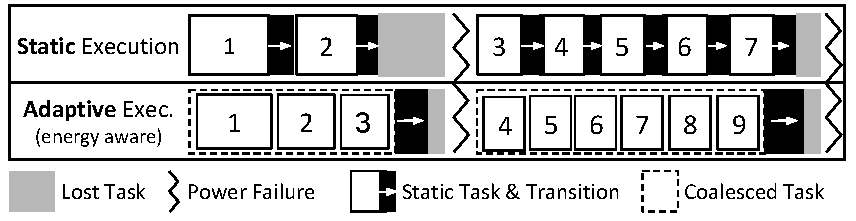
\includegraphics[width=0.5\columnwidth]{figures/coal_Intro_Figure.pdf}
% 	\caption{When $N$ tasks coalesced $N-1$ commit operations are skipped.}
% 	\label{fig:coalIntro}
% \end{wrapfigure}

When incoming energy is sufficient to run multiple consecutive tasks,
committing state after each task is wasteful. \sys mitigates this
waste by deferring the expensive commits and performing them in a
batch. In the resulting execution, several tasks are \emph{merged} into a
single virtual task---a process we call \emph{coalescing}. 
%
When $N$ tasks are coalesced, $N-1$ boundaries are crossed and some number of
pages are dirtied. The first $N-2$ executions of \transition statement skip
committing dirty pages to non-volatile memory, leaving the work of committing
pages modified by any of the $N$ tasks to the statement $N-1$.
Coalescing reduces the total number of non-volatile memory
accesses, because when coalesced tasks access the same pages of data, only the
last version of the page needs to be committed.  
\textcolor{red}{maybe is possible to demonstrate with data? count number of executed non-volatile vs volatile accesses}
%
\textbf{Trade-off between Speed and Wasted Effort.} \sys can coalesce an
arbitrary number of consecutive tasks. However, as more tasks coalesce, their
collective commit overhead amortizes better, but the risk of wasting work also
increases. If power fails during a long sequence of coalesced tasks, execution
will restart from the last commit, i.e. the first task in the sequence, losing
the progress made by any of the coalesced tasks.  The challenge to coalescing
tasks is determining how many tasks to coalesce before committing.
%
%During execution, an executing task is either a {\em coalesced} task, which
%does not commit its state before transitioning or a {\em committing} task,
%which does commit its state before transitioning.

\textbf{Task Coalescing Strategies.} 
%
\begin{algorithm}[t]
	\caption{Coalescing}
	\label{algo:genCoalescing}
	\scriptsize
	%\small
	\begin{algorithmic}[1]
        \State $H_\text{p} \gets H_\text{c}$
        \State $H_\text{p} \gets 0$ 
        \State $H_\text{B} \leftarrow $ \Call{$f_\text{reboot}$}{B, $H_\text{p}$}

        \While{$\texttt{true}$}
	        \State $ B_\text{c} \gets B$
	        %
	        \While{$ B_\text{c} > 0$}
		        \State \Call{execute\_task}{$T_\texttt{i}$}
		        \State $W \leftarrow $ \Call{$f_\text{weight}$}{$T_\text{i}$}
		        \State $B_\text{c} \gets B_\text{c} - W$
				\State $H_\text{c} \gets H_\text{c} + W$
	        \EndWhile
	        %
	         \State $B \leftarrow $ \Call{$f_\text{compl}$}{B, $H_\text{c}$,$H_\text{p}$}
	        \State \Call{commit\_to\_fram}{\null}
        \EndWhile
	\end{algorithmic}
\end{algorithm}
%
%
The likelihood that a task group will complete depends on the total amount of
energy consumed by all tasks in the group, i.e. the size of the dynamic task.
%
A good coalescing strategy must moderate the risk of wasted work and capitalize
on benefits of deferred commits by adapting the target size of the dynamic task
to the energy available at runtime. 
%
To describe the proposed strategies we will use the following parameters:
\begin{itemize}
\item target budget $B$: total number of static tasks to be coalesced.
\item current budget $B_\text{c}$: remaining number of tasks to be coalesced before committing to non-volatile memory; 
\item history $H$: up on reboot, it is the number of executed static tasks between the last two power interrupts. While executing, it is the number of executed static tasks since the last power interrupt.
\end{itemize}

%% Coalescing motivation

% Finding an optimal task size, given random energy conditions is an open question. Obviously, a static approach does not have the potential to answer it. Therefore, \sys champions runtime-based methods to approximate the ideal task size under random energy shots arrival. Furthermore, \sys advocates making intermittently powered software energy-aware is the key for \emph{efficient code execution and probability}. 
 

% %% address the challenge and define the optimal task

% \sys advances its execution in a state-less (or virtual) manner, and then it frequently saves its forward progress. The longer \sys virtually progresses, the less committing (saving data to non-volatile memory) overhead it introduces. However, long state-less execution results in a considerable re-execution penalty---all the tasks that have been virtually executed must be re-executed after a power interrupt. As such, an optimal task is a task that occupies with a single commit an entire power cycle, which is therefore necessarily of a varying length.  

% %% How does Coala approximates an ideal task


The general structure of the proposed coalescing strategies is summaries in algorithm~\ref{algo:genCoalescing}, where where $H_\text{p}$, $H_\text{c}$, $B$ and $B_\text{c}$ represent past history, current history, target budget and current budget, respectively. $T_\text{i}$ is the i-th task being executed and $W$ is its weight.
A coalescing strategy and its performance are defined by the functions:
\begin{itemize}
\item $f_\text{reboot}$: which updates the target budget after a reboot.
\item $f_\text{weight}$: which returns the weight of the task just executed and its unit. 
\item $f_\text{compl}$ : which updates the target budget after a successful completion of a dynamic coalesced task.
\end{itemize}
The following sections detail the different strategies \sys proposes and the needs that originated from one strategy leading to the conception of another one.

\subsubsection{Energy-blind Coalescing}
\label{subsec:energyBlind}

\begin{wrapfigure}{t!}{0.5\textwidth}
	\centering
	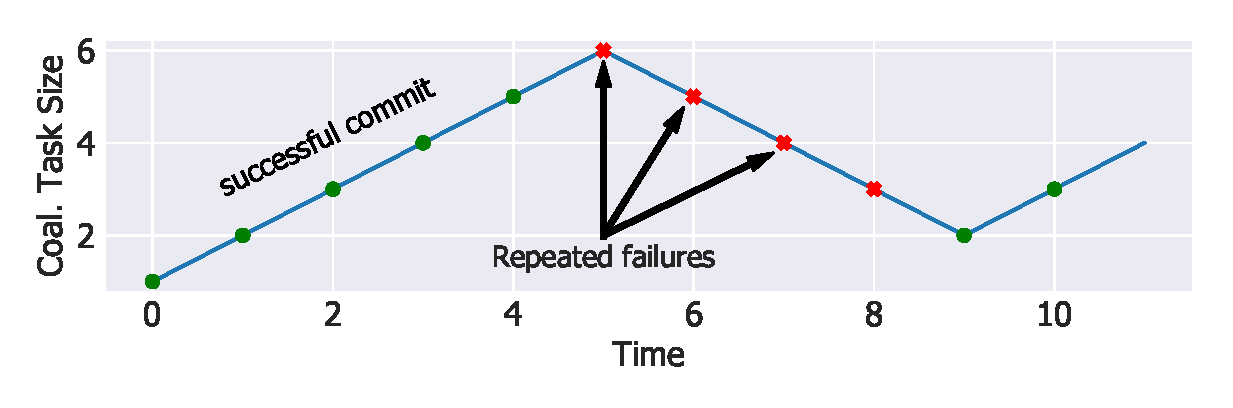
\includegraphics[width=0.5\columnwidth]{figures/slowCoal}
	\caption{The {\em energy blind coalescing} algorithm \emph{linearly} updates its coalescing target.}
	\label{fig:slowCoal}
\end{wrapfigure}

The need for \emph{adaptiveness}, that is coalescing static tasks, can be fulfilled by a naive strategy, having the target budget $B$ to increase by $x$ static tasks after a successful completion of a coalesced task, and to decrease by the same number of tasks upon a reboot. In this case: 
\begin{itemize}
\item $f_\text{reboot}(B, H_\text{p}) = B - x $;
\item $f_\text{weight}(T_\text{i}) =  1$; 
\item $f_\text{compl}(B,H_\text{c},H_\text{p}) = B + x$; 
\end{itemize}
Due to the linear behavior of the target adaptation, this algorithm is slow in reacting to the changes in energy conditions; the energy required by a coalesced task or the available energy. In particular, this algorithm can experience a large number of \emph{repeated power} failures without forward progress. 

\subsubsection{Energy-aware Coalescing}
\label{subsec:ECoalescing}
This algorithm tunes its target budget based on the recent history of execution. It takes advantage of the guarantees that the energy buffer offers on a fresh start by coalescing many static tasks. Then it approaches the expected power failure carefully by reduces the task target size by x\%, amongst 25\%, 50\% and 75\% the 50\% shows the best performance and therefore it is the default of \sys. If the algorithm concludes that it wrongly estimated the time of the power failure, it will force target re-tuning based on the new history of execution. 


\begin{wrapfigure}{}{0.5\textwidth}
	\centering
	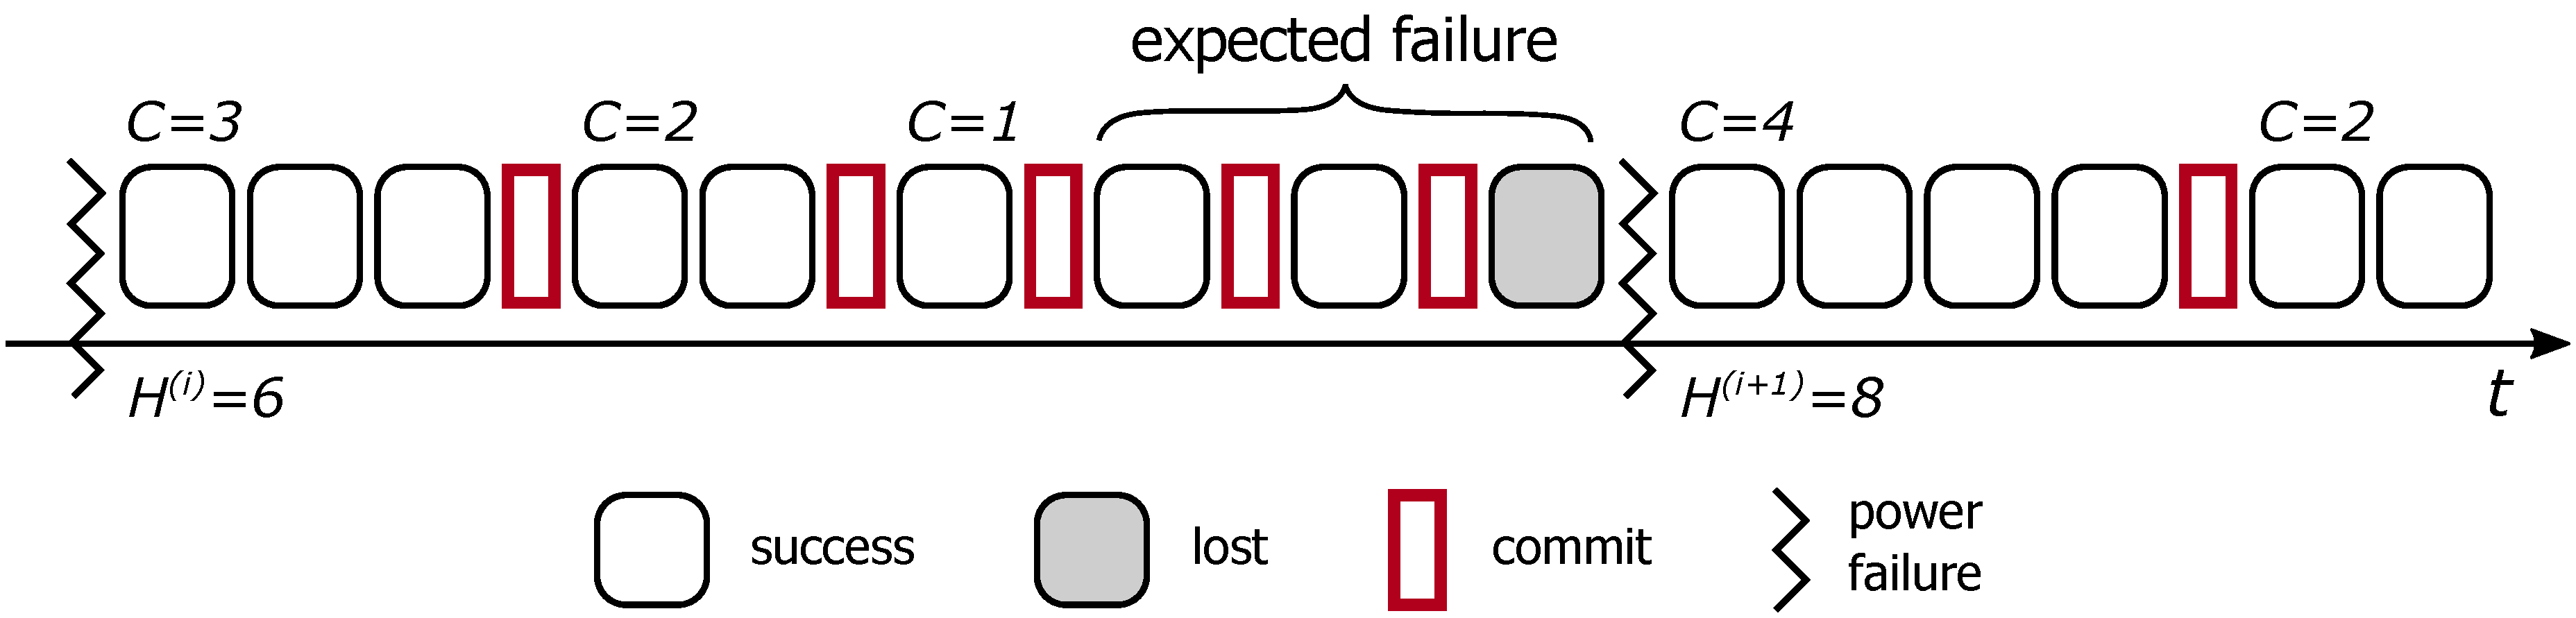
\includegraphics[width=0.5\columnwidth]{figures/energy-aware-coal.pdf}
	\caption{placeholder}
	\label{fig:energyAware}
\end{wrapfigure}
































